\documentclass[12pt,oneside,a4paper]{article}

\usepackage{./top/custom}

\usepackage[backend=biber]{biblatex}
\addbibresource{./top/biblio.bib}
\setcounter{tocdepth}{3}

\lstset{language=Julia}

% new commands (fold)
\newcounter{nalg}[section] % defines algorithm counter for chapter-level
\renewcommand{\thenalg}{\thechapter .\arabic{nalg}} %defines appearance of the algorithm counter
\DeclareCaptionLabelFormat{algocaption}{Algorithm \thenalg} % defines a new caption label as Algorithm x.y

\lstnewenvironment{algorithm}[1][] %defines the algorithm listing environment
{   
    \refstepcounter{nalg} %increments algorithm number
    \captionsetup{labelformat=algocaption,labelsep=colon} %defines the caption setup for: it ises label format as the declared caption label above and makes label and caption text to be separated by a ':'
    \lstset{ %this is the stype
        frame=tB,
        numbers=left, 
        numberstyle=\tiny,
        basicstyle=\scriptsize, 
        keywordstyle=\color{black}\bfseries\em,
        keywords={,input, output, return, datatype, function, in, if, else, foreach, while, begin, end, } %add the keywords you want, or load a language as Rubens explains in his comment above.
        numbers=left,
        xleftmargin=.04\textwidth,
        #1 % this is to add specific settings to an usage of this environment (for instnce, the caption and referable label)
    }
}
{}
% new commands (end)

\begin{document}
\begin{titlepage}
\begin{center}

%
\includegraphics[scale=0.5]{./img/logo_centralesup.jpg} \hfill
%
\includegraphics[scale=0.3]{./img/logo_digiplante.png}

\vfill 

\textsc{\Large Projet enjeu : Santé et biotechnologies}\\[0.5cm]

\vfill

\textsc{\Large Rapport final}\\[1.5cm] 

% Title
\HRule \\[0.4cm]
{ \LARGE \bfseries Développement d'outils mathématiques \\ 
   pour l'agriculture de précision \\[0.4cm] }

\HRule \\[1.5cm]

\vfill

{\large
\begin{center}
  \textbf{Client et Référent Pédagogique} \\~\\
\begin{tabular}{rl}
   \quad Pierre &\textsc{Carmier} \\
    \quad Paul-Henry &\textsc{Courn\`ede} \\
  
\end{tabular}
\end{center}
\vfill
\begin{center}
  \textbf{P2018 : groupe SBT-11} \\~\\
  
\begin{tabular}{rl}

    \quad John &\textsc{de Wasseige} \\
    \quad Nayef &\textsc{Derwiche} \\
    \quad Alexis &\textsc{Mathey} \\
    \quad Daina &\textsc{Zheng} \\ \\
\end{tabular}
\end{center}
}

\vfill

{\large 10 juin 2015}

\end{center}
\end{titlepage}

\tableofcontents
\newpage

\section*{Résumé}
\addcontentsline{toc}{section}{Résumé}
Ce rapport présente nos résultats et nos perspectives
du projet et s'articule autour de cinq parties.

Dans un premier temps, nous introduisons le contexte global du
projet en mettant l'accent sur l'objectif poursuivi par celui-ci.

On expose ensuite une synthèse de l'\emph{étude documentaire}
en décrivant brièvement chacun des thèmes abordés dans celle-ci.
On rappelera notamment quelques notions de physiologie des plantes, un bref historique de la modélisation des plantes
ainsi que les principaux modèles actuels et leurs caractéristiques communes.

La partie suivante décrit l'ensemble des méthodes
utilisées pour mener à bien notre projet.
On décrira d'abord les outils de travail que nous avons
utilisés afin de collaborer efficacement.
On rappelera ensuite la façon dont nous avons
géré notre bibliographie.
Un planning de la répartition des tâches à travers
le semestre sera ensuite donné.
On terminera cette partie en décrivant de façon
exhaustive les difficultés que nous avons rencontrées
jusqu'à maintenant.

Avant de décrire les résultats obtenus,
nous rappelerons de manière synthétique le fonctionnement
de notre modèle.
On expliquera ensuite comment nous avons implémenté
celui-ci en \textsc{Julia} en détaillant les
variables et fonctions utilisées.

La dernière partie reprendra d'une part nos résultats
ainsi qu'une analyse de ceux-ci et de leur pertinence
par rapport à ce que l'on observe expérimentalement,
et d'autre part les perspectives à long terme
que nous proposons pour le projet.

\newpage
\section{Introduction}
\newpage


\section{Code et modèle}
\subsection{Description du modèle}

Le modèle LNAS blé est une version plus complexe du modèle LNAS betterave. Le modèle est constitué de deux compartiments principaux : le compartiment circulation de biomasse et le compartiment simulation de l'eau. Dans cette section nous ferons une explication des principes généraux et une description qualitative du modèle. Le lecteur intéressé trouvera tous les détails en annexe~\ref{ann:articlePierre} dans  la référence que nous avons nous-même utilisé pour implémenter le modèle.

\subsubsection{Circulation de biomasse}

\begin{figure}[H]

\begin{center}
 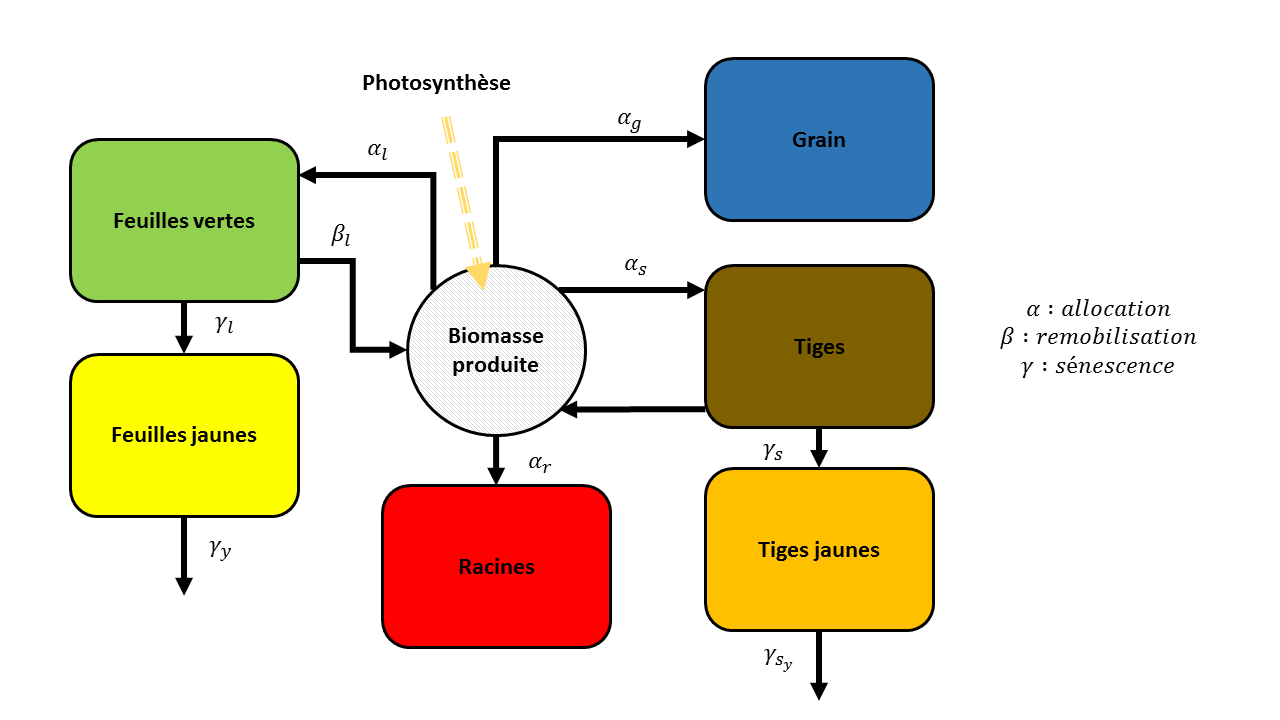
\includegraphics[scale = 0.42]{./img/modelSchema.png}
 \caption{Schéma de la circulation de biomasse.}
 \label{fig:schemaModel}
\end{center}

\end{figure}

Le modèle va à chaque itération calculer la quantité de biomasse produite, l'ajouter à un pool de biomasse. Ensuite il va calculer des coefficients d'allocation, de remobilisation et de sénescence qui vont déterminer la circulation de biomasse entre les différents compartiment, la loi de conservation voulant que toute la biomasse soit allouée au final. 
Les coefficients d'allocations déterminent la part de biomasse distribuée à chaque compartiment. Les coefficients de sénescence représentent un processus de vieillissement. Les coefficient de remobilisation représentent la part de biomasse des compartiment retournée au pool de biomasse pour être à nouveau alloué.

Les étapes sont les suivantes : 

\begin{itemize}

\item La biomasse est produite par photosynthèse et la quantité crée est calculée grâce à la loi de Beer-Lambert.  Un coefficient de stress hydrique et un coefficient de stress thermique peuvent réduire la production.

\item Des coefficients d'allocation sont ensuite calculés selon des lois log-normales, avec pour paramètres un temps caractéristique, à partir duquel l'allocation commence à être significative, une espérance et une variance. Typiquement, l'allocation aux racines et aux feuilles domine au départ, puis c'est celle aux tiges et vers la maturité de la plante c'est cella au grain.

\item Des coefficients de sénescence sont calculés selon des lois log-normales de la même façon. La sénescence des feuilles commence vers la fin de la croissance de la plante.

\item Enfin, des coefficients de remobilisation sont calculés toujours selon des lois log-normales. La remobilisation intervient de façon intense vers la fin pour les feuilles et les tiges en faveur du grain.

\end{itemize}

La valeur critique qui donne le rythme d'évolution de la plante n'est pas le temps réel mais le temps thermique qui correspond à l'accumulation de températures dépassant un certain seuil :
\[
\tau^{(n+1)} = \tau^{(n)} + \max[0, \underline{T^{(n)}} - T_c], 
\]
L'idée part d'un constat simple : la croissance de la plante est ralentie lorsque la température est basse.

\subsubsection{Simulation de l'eau}

\begin{figure}[H]

\begin{center}
 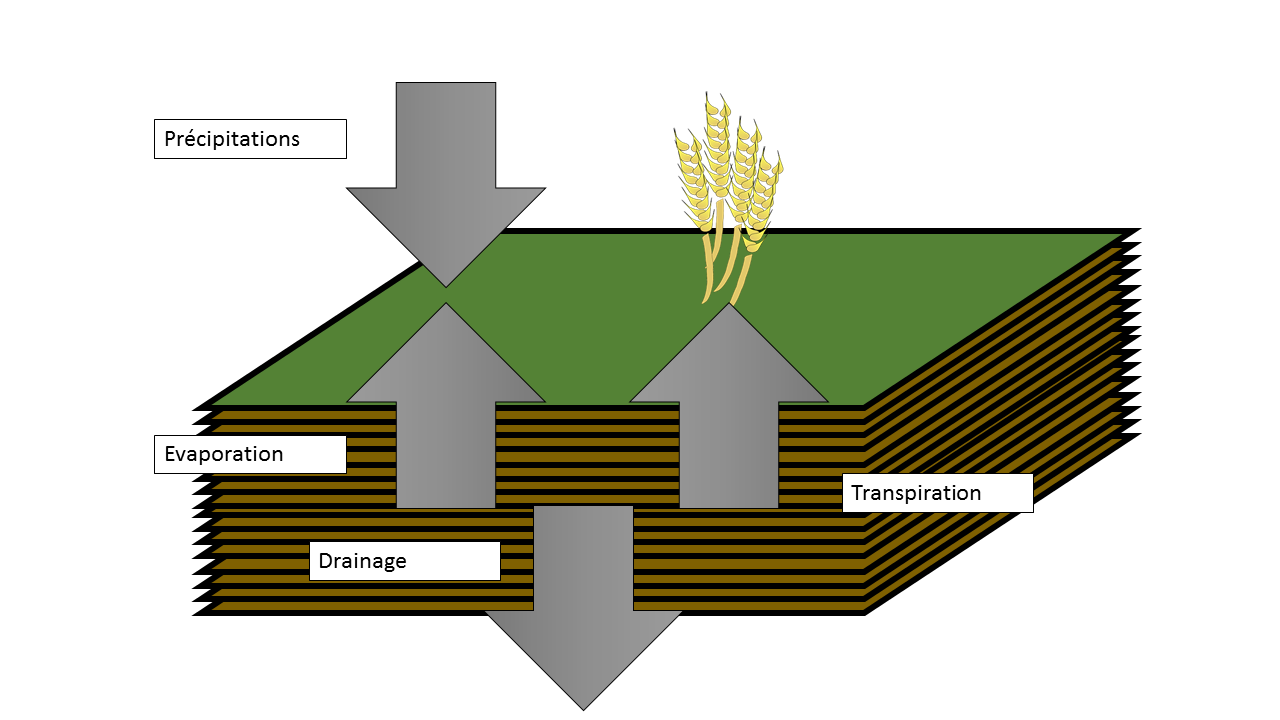
\includegraphics[scale = 0.42]{./img/waterSchema.png}
 \caption{Schéma de simulation de l'eau}
 \label{fig:waterModel}
\end{center}

\end{figure}

La simulation de l'eau est assez précisément décrite dans le modèle
et la figure~\ref{fig:waterModel} permet de comprendre intuitivement ce qu'il se passe. 

Elle repose sur l'équation d'équilibre de l'eau
\[ R^{(n+1)} = R^{(n)} + W^{(n)} - Es^{(n)} - Tp^{(n)} - d^{(n)}\]

Dans cette équation, $W^{(n)}$ représente les précipitations quotidiennes,
$Es^{(n)}$ est la quantité d'eau perdue par évaporation,
$Tp^{(n)}$ est la quantité d'eau transpirée par la plante 
et $d^{(n)}$ est une fonction de drainage qui évacue l'eau ne pouvant être absorbé si le sol est saturé. 

On calcule l'évaporation et la transpiration potentielles, qui sont la quantité d'eau pouvant être évaporée et transpirée en fonction de l'environnement (evapotranspiration du milieu, ensoleillement...). 
Puis l'évaporation et la transpiration ``max'' qui sont celles requises étant donnée la plante et l'environnement (profondeur des racines, ensoleillement...). 
On regarde donc la transpiration et l'évaporation qui aura effectivement lieu, qui sera le minimum entre le potentiel et ce qui est demandé.
Si la transpiration requise pour la plante n'est pas satisfaite, il y aura un stress hydrique. 

Une fois l'évaporation et la transpiration déterminée on rajoute au sol l'eau apportée par les précipitations puis on enlève l'eau évaporée puis transpirée. Les apports et pertes d'eau se font en FIFO (First In, First Out) ou ``piles'' : l'eau est d'abord rajoutée sur les couches supérieures jusqu'à saturation à l'humidité maximale (humidité au delà de laquelle le sol ne peut plus absorber d'eau) avant d'être rajoutée aux couches les plus basses, de même, on retire l'eau des couches supérieures d'abord jusqu'à atteindre l'humidité minimale (humidité en deçà laquelle on ne peut plus tirer d'eau), avant de retirer l'eau des couches les plus basses.
Tout excès éventuel d'eau après opérations est drainé.
\newpage
\subsection{Description du fonctionnement du code}
Dans un premier temps, nous avons construit un modèle informatique à partir
du modèle mathématique fourni~\cite{lnas_model_wheat}.

Il s'agissait d'abord d'affecter à chaque variable du modèle un représentant
dans notre programme, en rendant ces derniers assez explicites
afin d'être plus efficace pour l'implémentation des fonctions.
Les tableaux~\ref{table:state_var},~\ref{table:control_var} et~\ref{table:param_var}
contiennent respectivement les variables d'\emph{état}, temporaires, auxiliaires et principales, 
les variables \emph{environnementales} et les \emph{paramètres} de la tige, du sol et des racines.

La deuxième partie du travail consistait à définir les différentes fonctions (appelées ``modules'' selon les conventions Pygmalion)
qui mettent à jour les variables d'état et paramètres du 
temps $n$ au temps $n+1$.
L'implémentation de chacune d'entre elles est basée sur l'algorithme générique~\ref{lst:genfun}.
On retrouve à l'entrée les variables d'états \texttt{xn} et \texttt{xnplus1},
le temps \texttt{n}, les variables de contrôles \texttt{u}, les paramètres \texttt{p}.
On va ensuite mettre à jour une composante de \lstinline|xnplus1| par rapport à \texttt{xn} en fonction de \texttt{n}, \texttt{u} et \texttt{p} en suivant la description du modèle.

\begin{algorithm}[h]
  \caption{Algorithme générique qui sert de base pour l'implémentation
des fonctions. La fonction $f$ n'est pas définie mais sert de placeholder
pour représenter les opérations nécessaires à la mise à jour de \lstinline|xnplus1|.}
\label{lst:genfun}
  \begin{algorithmic}[1]
    \Procedure{Generic}{int $n$, State Vector $xn$, Control Vector $u$, Parameters Vector $p$, State Vector $xnplus1$}
    \State \textbf{begin}
      \State $xnplus1.composante \gets f(p.composante, u.composante, xn.composante)$
    \State \textbf{end}
    \State \textbf{return} None
    \EndProcedure
  \end{algorithmic}
\end{algorithm}

\lstset{        literate=
                       {==}{$={}$}{1}}

À titre d'exemple, on présente la fonction \lstinline|get_pot_evaporation| qui met
à jour l'évaporation requise en fonction des conditions environnementales
selon l'équation~\ref{eq:req_evap}.
\begin{equation}
  \text{Espot}^{(n)} = K_s \text{ ET0 } e^{-\lambda \text{ LAI}^{(n)}}
  \label{eq:req_evap}
\end{equation}
On obtient en \textsc{Julia} l'implémentation suivante
\begin{lstlisting}
function get_pot_evaporation!(n, xn, u, p, xnplus1)
  xnplus1.soil_req_evaporation = 
    p.k_s * u.ET0[n] * exp( -p.lambda * xn.leaf_area_index) 
end
\end{lstlisting}

Il reste finalement deux fonctions particulières qui ne suivent
pas l'algorithme~\ref{lst:genfun}.
% Elles se nomment \lstinline|initialize|, \lstinline|transition|
% et servent respectivement à initialiser \lstinline|xn| et
% à exécuter toutes les fonctions pour passer au temps suivant.

\begin{enumerate}
  \item \lstinline|initialize| qui va initialer les composantes de \lstinline|xn|,
  \item \lstinline|transition| qui permet de passer au temps suivant et d'exécuter toutes les fonctions.
\end{enumerate}




\begin{table}[h]
  \centering
  \begin{tabular}{c|c}
    \textbf{Modèle mathématique} & \textbf{Implémentation} \\
    $Q_r$ & root\_biomass \\
    $Q_s$ & stem\_biomass \\
    $Q_l$ & green\_leaf\_biomass \\
    $Q_g$ & grain\_biomass \\
    $Q_y$ & yellow\_leaf\_biomass \\
    $\theta$ & soil\_humidity \\
    $\tau$ & thermal\_time \\
    $R$ & soil\_contained\_water \\
    $E_s$ & soil\_water\_evaporated \\
    $T_p$ & water\_transpired \\
    $z_r$ & root\_horizon \\
    SSI & stomatal\_stress\_index \\
    TSI & thermal\_stress\_index \\
    TSI$_{\uparrow}$ & thermal\_stress\_index \\
    TSI$_{\downarrow}$ & soil\_thermal\_stress\_index \\
    % Auxiliary
    $q$ & produced\_biomass \\
    LAI & leaf\_area\_index \\
    E\textsubscript{spot} & soil\_req\_evaporation \\
    T\textsubscript{ppot} & req\_transpiration \\
    E\textsubscript{smax} & soil\_max\_evaporation \\
    T\textsubscript{pmax} & max\_transpiration \\
    T$_{\downarrow}$ & soil\_temperature \\
    % Temporary
    $\alpha_g$ & alpha\_g \\
    $\alpha_s$ & alpha\_s \\
    $\alpha_r$ & alpha\_r \\
    $\alpha_l$ & alpha\_l \\
    $\beta_s$ & beta\_s \\
    $\beta_l$ & beta\_l \\
    $\gamma_l$ & gamma\_l \\
    $\gamma_y$ & gamma\_y \\
  \end{tabular}
  \caption{Variables d'\emph{état} du modèle mathématique et leurs noms
  dans l'implémentation.}
  \label{table:state_var}
\end{table}

\begin{table}
  \centering
  \begin{tabular}{c|c}
    \textbf{Modèle mathématique} & \textbf{Implémentation} \\
    $T$ & vec\_ext\_temperature \\
    PAR & vec\_par \\
    $W$ & vec\_water\_input \\
    ET0 & vec\_et0 \\
  \end{tabular}
  \caption{Variables de \emph{contrôle} du modèle mathématique et leurs noms
  dans l'implémentation.}
  \label{table:control_var}
\end{table}

\begin{table}
  \centering
  \begin{tabular}{c|c}
    \textbf{Modèle mathématique} & \textbf{Implémentation} \\
    $t_c$ & t\_c \\
    $t_{opt}$ & t\_opt \\
    $\mu_g$ & mu\_g \\
    $\sigma_g$ & sigma\_g \\
    $\eta_s$ & eta\_s \\
    $\eta_l$ & eta\_l \\
    $\tau_l$ & tau\_l \\
    $\mu_l$ & mu\_l \\
    $\sigma_l$ & sigma\_l \\
    $\tau_y$ & tau\_y \\
    $\mu_y$ & mu\_y \\
    $\sigma_y$ & sigma\_y \\
    RUE & rue \\
    $\lambda$ & lambda \\
    $\rho_l$ & rho\_l \\
    $K_c$ & k\_c \\
    $K_s$ & k\_s \\
    $\theta_{max}$ & theta\_max \\
    $\theta_{min}$ & theta\_min \\
    $z_s$ & z\_s \\
    $z_m$ & z\_m \\
    $\rho_r$ & rho\_r \\
    $t_{\downarrow c}$ & t\_soil\_c \\
    $t_{\downarrow opt}$ & t\_soil\_opt \\
  \end{tabular}
  \caption{Paramètres du modèle mathématique et leurs noms
  dans l'implémentation.}
  \label{table:parameters_var}
\end{table}
  








\subsection{Estimation des paramètres}

Maintenant que le modèle est implémanté, il faut pouvoir estimer les paramètres qui interviennent dans le modèle, pour pouvoir utiliser le dit modèle.

Pour cela, nous utilisons une méthode déjà implémentée sur la plateforme ``lgs'', pour Generalized Least Squares (méthode des moindres carrés généralisée).

A partir des données expérimentales d'un champ de blé par exemple, cette méthode cherche les valeurs, les paramètres qui font converger les valeurs mesurées et les valeurs calculées par le modèle. 
La méthodes des moindres carrés généralisée est une méthode classique pour l'estimation de paramètres dans le cas de modèles déterministes, et c'est la cas ici puisque nous n'avons pas implémenté de bruit aléatoire dans notre modèle.

La méthode minimise la probabilité que les données expérimentales soient différentes de ce qui est prédit par le modèle. 
Mais, les calculs ne peuvent être conduits qu'en affectant une valeur arbitraire aux paramètres. On obtient ainsi une nouvelle valeur des paramètres, avec lesquelles on calcule de nouvelles valeurs des paramètres. Et ainsi de suite, jusqu'à que la valeur des paramètres converge.

L'avantage de cette méthode est son efficacité pour déterminer rapidement et avec une assez bonne précision les valeurs cherchées.
De plus, le fait que cette méthode soit déjà implémentée sur la plateforme est un autre avantage, puisque cela nous permet de l'utiliser sans avoir à l'implémenter. 


\newpage
\subsection{Markov}

Ces modèles sont des \emph{modèles de Markov} à temps discret. 
Soit $(t_{n}) n \in [0,N]$, la séquence finie des temps successifs correspondants
aux étapes de l’évolution. On note $X_{n}\in \reels^d$
l'ensemble des variables caractéristiques du système à $t_{n}$, $U_n \in \reels^u$
l'ensemble des variables exogènes (entrées, contrôle...) à $t_{n}$,
et $P\in R^p$ le vecteur de paramètres du modèle.
Comme pour la plupart des systèmes biologiques, $X_{n}$ peut ne pas être
complètement accessible à l'observation, et on note donc $Y_n \in \reels^{q_n}$
l'ensemble observé/mesuré des variables au temps $n$.
On note $Y=Y_n, n \in [0,N]$.
La fonction de densité initiale pour $X_0$ est $\mu_p$ 
et la densité de transition de Markov est $f_{n,P,U_n}$ :

\[
	X_0 \sim \mu_p \quad \text{ et } \quad
	 X_{n+1} \mid (X_n=x) \sim f_{n,P,U_n}(.\mid x)	\quad \forall n \in [0;N-1]
\]

L'observation $Y_n$ dépend de $X_n$ et la densité conditionnelle 
est donnée par $g_{n,P}$:
\[Y_n \mid (X_n = x) \sim g_{n,P} \]

Ce cadre stochastique permet d'aboutir et de décrire les modèles dynamiques discrets déterministes, en écrivant : 
\[
\left\{
    \begin{array}{ll}
        X_{n+1} &= F_n(X_n,U_n,P) \\
        Y_n &= G_n(X_n,P)
    \end{array}
\right.
\]

describes how an important category of plant growth models can be set in this framework. For example, for functional-structural models that describe biomass budget during plant growth (see for example LIGNUM [52] or GREENLAB [46]), the state variables correspond to daily biomass accumulation and to masses of plant organs according to their categories, the parameters are genotype specific, and the external variables Un correspond to environmental variables (radiation, temperature, soil water content ...).

Generally, not all the state variables can be observed experimentally (for example daily biomass pro- duction) and the experimentation being heavy (specifically when it comes to the masses of individual organs), observations are not done at all time steps. If we denote by O the set of all time step indexes corresponding to observation stages:
\[
  \mathcal{O} = \left\{i \in [1; N ] \text{ où } 
  t_i \text{ est un temps d'observation}\right\} 
\]
we then have qi > 0 if and only if i  O (where we recall that qi is the dimension of Yi). Note also that the non-zero qi have no reason to be identical (as illustrated for example in [45] for a model of maize growth, in which at some stages individual plants were measured at organ level, and at other stages only compartment data were available, corresponding to different Gi).

%1.1 Processus de Markov :
%
%Définition 1 : Le processus 〖〖(X〗_t)〗_(t≥0) est dit de Markov, si :
%	Pour tout t_1<t_2…< t_(n+1), pour tout x_1,…,x_(n+1)  :
%P(X_(t_(n+1) )=x_(n+1)∕X_(t_1 )=x_1,…,X_(t_n )=x_n )=P(X_(t_(n+1) )=x_(n+1)⁄X_(t_n ) =x_n)
%	Pour tout s et t, pour tout x,y∈E, P(X_(t+s)=y⁄X_s =x) ne dépend que de t.
%
%Remarque : L’axiome (1) (axiome de Markov) traduit que la probabilité de n’importe quel comportement futur, le présent étant connu, n’est pas modifié par toute connaissance supplémentaire du passé.

\newpage

\section{Conclusion}

\newpage
\section*{Remerciements}
\addcontentsline{toc}{section}{Remerciements}

Nous tenons tout d'abord à remercier notre client Pierre Carmier,
pour sa pédagogie et son temps précieux accordé. 
Nous remercions également Mme Le Chevalier et Mme Lopes, qui encadrent
le projet de façon motivante et efficace.
Leurs remarques et retours sur nos présentations 
ainsi que sur l'avancement de notre projet
nous ont été très utiles pour prendre le recul
nécessaire à la rédaction de ce rapport.
Enfin, merci à nos responsables d'ateliers Mme Lévy et M. Bertrand, qui nous ont permis de mieux appréhender l'aspect humain du projet, que ce soit pour présenter à l'oral ou communiquer au sein du groupe.
\newpage

\addcontentsline{toc}{section}{Bibliographie}
\nocite{*}
\printbibliography
\newpage

\end{document}